\section{Graphical user interface}
The purpose of the graphical user interface is to simplify the usage of ENVISIoN. 

\subsection{Start-up}
When the user run the application a window opens, see figure \ref{fig:GUIStartup}. After ENVISIoN has been opened, two possible menu-choices appear, ``Parser'' and ``Visualization''.

\begin{figure}[ht]
    \centering
    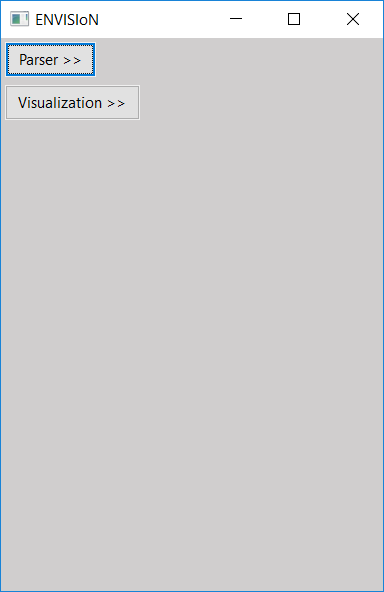
\includegraphics[angle=0,scale=0.5]{images/GUIBasWin.png}
    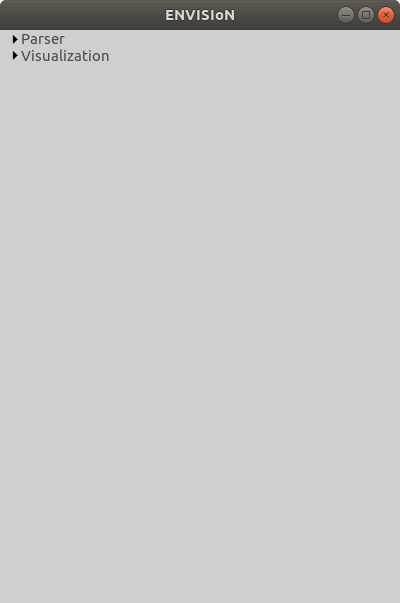
\includegraphics[angle=0,scale=0.49]{images/GUIBasLinux.png}
    \caption{ENVISIoN start up-window, for Windows on the left and Linux on the right.}
    \label{fig:GUIStartup}
\end{figure}

\subsection{Parser menu}
The parser menu is localized on top in the interface. To access its content, press the fold out button to expand the menu. The result will be that of figure \ref{fig:GUIParserWindows}, depending on the system running the software. 


\begin{figure}[ht]
    \centering
    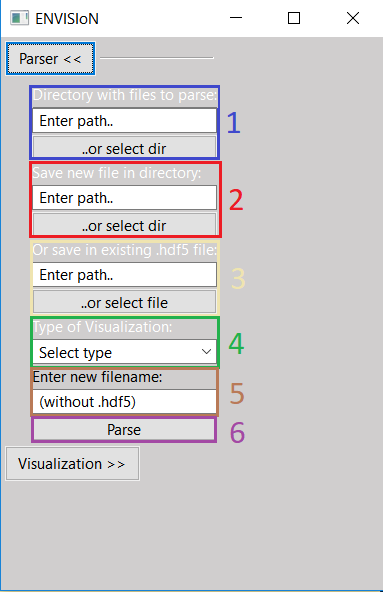
\includegraphics[angle=0,scale=0.6]{images/GUIParser.png}
    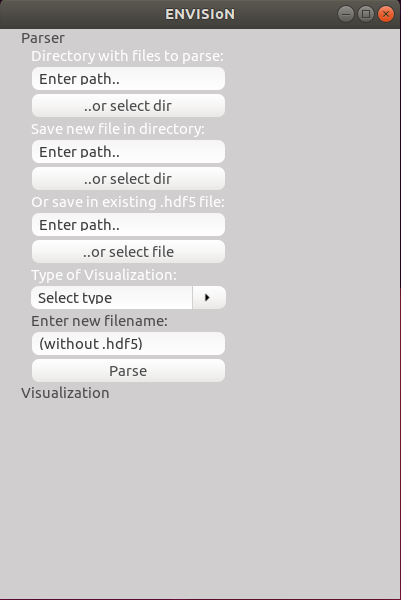
\includegraphics[angle=0,scale=0.356]{images/GUIParserLinux.png}
    \caption{Parser menu expanded, for Windows on the left and Linux on the right.}
    \label{fig:GUIParserWindows}
\end{figure}

For quick step-by-step guide, scroll down to last segment of this subsection.\newline

In the blue box, labeled ``1'', the path to the directory of VASP-files to parse is selected. There are two options, either the path can be entered as a string in the text field or the ``..or select dir''-button can be pressed. This button will reveal the file explorer and allow to select the desired folder.

In the red box, labeled ``2'', the path to the desired saving directory for the new hdf5-files is selected. This path-selection has the same two options as the previous.

In the yellow box, labeled ``3'', the path to an existing hdf5-file can be selected. Here, there are two options as well, which are similar to those above. The difference is that the button will open a file explorer where an hdf5-file shall be selected.

In the green box, labeled ``4'', the type of the parsing for certain visualizations can be picked. If one type of visualization is desired, there can be of advantage to pick that in the drop-down list to enhance performance of the parser. If not changed or if ``All'' is selected, the parser will run all possible types of parsing.
The available choices for types are:
\begin{itemize}
    \item All
    \item Bandstructure
    \item Charge
    \item DoS - Density of States
    \item ELF - Electron Localization Function
    \item Fermi Energy
    \item MD - Molecular Dynamics
    \item Parchg - Partial Charge
    \item PCF - Pair Correlation Function
    \item Unitcell
\end{itemize}

In the brown box, labeled ``5'', if a new hdf5-file is to created, the name of the new file is entered here without file extension.

In the purple box, labeled ``6'', is the execution-button of the parser. When pressing this button the parser tries to run. Afterwards, a message box will appear on the screen with the status of the parsing. If the parsing was successful the message box will show for which data the parsing was done. If it failed, the message box will tell where it failed. If no message box appear, then something went wrong that wasn't detected, an exception that wasn't caught.

\subsubsection{Quick Step-by-Step Guide}
For new *.hdf5 file:
\begin{enumerate}
    \item Enter path to directory in ``1''.
    \item Enter path to directory in ``2''.
    \item Select type in ``4''.
    \item Enter new file name in ``5''.
    \item Press ``Parse'' in ``6''.
    \item Message whether the parsing was successful or not will appear.
\end{enumerate}

For existing *.hdf5 file:
\begin{enumerate}
    \item Enter path to directory in ``1''.
    \item Enter path to file in ``3''.
    \item Select type in ``4''.
    \item Press 'Parse' in ``6''.
    \item Message weather the parsing was successful or not will appear.
\end{enumerate}


\subsection{Visualization menu}

\subsubsection{Common controls - Charge Density, ELF, and Partial Charge Density}
Because of the strong similarity between these three menues the interface share many elements. The common elements will be described here.

When opening any of the visualization main menues four sub-menues will be visible. \textit{Volume Rendering}, \textit{Volume Slice}, \textit{Atom Rendering} and \textit{Background}. All those control different aspects of the visualization.

\textbf{Volume Rendering menu}
\nyBild{instructions_volume.png}{Volume Rendering menu.}{instructions_volume}{1}
\begin{enumerate}[label={(\arabic*)}]
  \item Drop-down menu to choose volume shading mode. Affects how the volume is lighted.
  \item Toggle full transparency for volume densities lower than the lowest transfer function point.
  \item Edit existing transfer function points by editing text fields or picking color. Remove point by pressing ``-'' button.
  \item Add new transfer function point with specified value, alpha, and color by pressing ``+'' button.
  \item Click button to show volume density distribution histogram. Histogram will open in a new window.
  \item Click to save or load active transfer function. 
\end{enumerate}

\textbf{Volume Slice menu}
\nyBild{instructions_slice.png}{Slice menu.}{instructions_slice}{1}
\begin{enumerate}[label={(\arabic*)}]
  \item Text fields specify (x, y, z)-components of the normal vector of slice plane.
  \item Slider controls the height of the slice plane.
  \item Expandable menu to control the background of the slice image.
\end{enumerate}

\textbf{Atom Rendering menu}
\nyBild{instructions_atom.png}{Atom Rendering menu.}{instructions_atom}{1}
\begin{enumerate}[label={(\arabic*)}]
  \item Sliders to choose the radius of each atom type.
\end{enumerate}

\textbf{Background menu}
\nyBild{instructions_background.png}{Background menu.}{instructions_background}{1}
\begin{enumerate}[label={(\arabic*)}]
  \item Drop-down menu to choose the background pattern style.
  \item Select the two colors of the background. Either use the color picker on the left, or specify a RGBA-color via the text fields
  \item Button to swap positions of the colors.
  \item Drop-down menu to choose the blend mode of the background.
\end{enumerate}

\subsubsection{Charge Density}
\nyBild{instructions_charge.png}{Charge Density menu.}{instructions_charge}{1}
\begin{enumerate}[label={(\arabic*)}]
  \item Drop-down menu to select which band to visualize. Each band has its own volume data.
  \item Toggle the atom sphere rendering.
  \item Toggle the volume slice visualization.
  \item Expand the Volume Rendering menu.
  \item Expand the Atom Rendering menu.
  \item Expand the Background menu.
  \item Expand the Volume Slice menu.
\end{enumerate}

\subsubsection{ELF - Electron Localization Function}
\nyBild{instructions_elf.png}{ELF menu.}{instructions_elf}{1}
\begin{enumerate}[label={(\arabic*)}]
  \item Drop-down menu to select which band to visualize. Each band has its own volume data.
  \item Toggle the atom sphere rendering.
  \item Toggle the volume slice visualization.
  \item Expand the Volume Rendering menu.
  \item Expand the Atom Rendering menu.
  \item Expand the Background menu.
  \item Expand the Volume Slice menu.
\end{enumerate}

\subsubsection{Partial charge density}
\nyBild{instructions_parchg.png}{Partial charge density menu.}{instructions_parchg}{1}
\begin{enumerate}[label={(\arabic*)}]
  \item Manage selected bands and modes. Band selections and modes can be changed. Select ``None'' to remove band from visualization. 
  \item Add new band selection with selected mode. Select any other opetion than ''None'' to add new band to visualization.
  \item Toggle the atom sphere rendering.
  \item Toggle the volume slice visualization.
  \item Expand the Volume Rendering menu.
  \item Expand the Atom Rendering menu.
  \item Expand the Background menu.
  \item Expand the Volume Slice menu.
\end{enumerate}


\subsubsection{Bandstructure}
When expanding the bandstructure visualization menu the visualization starts and a control panel appears. This menu is shown in figure \ref{fig:GUIBand}.

\nyBild{GUIBand.png}{Bandstructure visualization menu expanded}{GUIBand}{0.6}

The bandstructure visualization menu contains a number of possibilities to control parameters.
\paragraph{Range and Scale: }
In the first (blue) box, controls for scaling and changing the visible interval appears. The range boxes sets minimum and maximum values for the axes to show. The scale box sets the scaling for the entire graph with maximum one and minimum at one over a hundred.
\paragraph{Help line: }
The help line, the blue line in the graph, is controlled by the red box in the graphical interface. By checking and unchecking the box, the help line is enabled and disabled. When the line is enabled, it is possible to move around to check which X-values corresponds to what part of the curve in the graph.
\paragraph{Grid: }
When grid is checked (yellow box) the visible mesh in figure \ref{fig:GUIBand} appears. The frequency of the grid lines is in direct relations to number of labels, covered in the next paragraph. The thickness of the lines is controlled from the text entry below the checkbox for the grid.
\paragraph{Labels: }
In the green box, the option of labels concerns if labels should be visible on the axes or not and the number of labels appearing along the axes. There is one option for each axis to show or hide the labels. The text entry is for number of labels apart from lowest value.
\paragraph{List of Y: }
Below the label ``List of Y'' in the brown box are controls for choosing lines to show and a list of all possible choices.The drop down list is not a control, it's a list of the possible bands to show. The tick box for ``Enable all Y'' enables all Y-values to be visualized or not. When enabled, the option to visualize some or one of the bands is disabled. 
The tick box for enabling y selection reveals a hidden text entry. Here it's possible to choose one or more band to visualize. The options of how to choose the lines are; ``n'', ``n:N'', ``n,N'' or some combination of these, where n and N are arbitrary integers corresponding to list indices. 

\subsubsection{DoS - Density of States}
When expanding the density of states visualization menu the visualization starts and a control panel appears. The menu is shown in figure \ref{fig:GUIDoS}.

\nyBild{GUIDoS.png}{Density of stats visualization menu expanded}{GUIDoS}{0.6}

\paragraph{Range and Scale: }
In the first, controls for scaling and changing the visible interval appears. The range boxes sets minimum and maximum values for the axes to show. The scale box sets the scaling for the entire graph with maximum one and minimum at one over a hundred.
\paragraph{Help line: }
The help line is controlled by the red box in the graphical interface. By checking and unchecking the box, the help line is enabled and disabled. When the line is enabled, it is possible to move around to check which X-values corresponds to what part of the curve in the graph.
\paragraph{Grid: }
When grid is checked the visible mesh in figure \ref{fig:GUIBand} appears. The frequency of the grid lines is in direct relations to number of labels, covered in the next paragraph. The thickness of the lines is controlled from the text entry below the checkbox for the grid.
\paragraph{Labels: }
The option of labels concerns if labels should be visible on the axes or not and the number of labels appearing along the axes. There is one option for each axis to show or hide the labels. The text entry is for number of labels apart from lowest value.
\paragraph{List of Y: }
Below the label 'List of Y' are controls for choosing lines to show and a list of all possible choices. Here, the drop down list is a control, which can select what line to show in the graph. The tick box for ``Enable all Y'' enables all Y-values to be visualized or not. When enabled, the option to visualize some or one of the bands is disabled. 
The tick box for enabling y selection reveals a hidden text entry. Here it's possible to choose one or more band to visualize. The options of how to choose the lines are; ``n'', ``n:N'', ``n,N'' or some combination of these, where n and N are arbitrary integers corresponding to list indices.

\subsubsection{PCF - Pair Correlation Function}
When expanding the PCF visualization menu the visualization starts and a control panel appears. In figure \ref{fig:GUIPCF}, this menu is visible.

\nyBild{GUIPCF.png}{Pair correlation function visualization menu expanded}{GUIPCF}{0.6}

\paragraph{Range and Scale: }
In the first, controls for scaling and changing the visible interval appears. The range boxes sets minimum and maximum values for the axes to show. The scale box sets the scaling for the entire graph with maximum one and minimum at one over a hundred.
\paragraph{Help line: }
The help line is controlled by the red box in the graphical interface. By checking and unchecking the box, the help line is enabled and disabled. When the line is enabled, it is possible to move around the line to check which X-values corresponds to what part of the curve in the graph.
\paragraph{Grid: }
When grid is checked the visible mesh in figure \ref{fig:GUIBand} appears. The frequency of the grid lines is in direct relations to number of labels, covered in the next paragraph. The thickness of the lines is controlled from the text entry below the checkbox for the grid.
\paragraph{Labels: }
The option of labels concerns if labels should be visible on the axes or not and the number of labels appearing along the axes. There is one option for each axis to show or hide the labels. The text entry is for number of labels apart from lowest value.
\paragraph{List of Y: }
Below the label ``List of Y'' are controls for choosing lines to show and a list of all possible choices. Here, the drop down list is a control, which can select what line to show in the graph. The tick box for ``Enable all Y'' enables all Y-values to be visualized or not. When enabled, the option to visualize some or one of the bands is disabled. 
The tick box for enabling y selection reveals a hidden text entry. Here it's possible to choose one or several bands to visualize. The options of how to choose the lines are; ``n'', ``n:N'', ``n,N'' or some combination of these, where n and N are arbitrary integers corresponding to list indices.

